\chapter{Implementation}
In the previous chapter we discussed some of the mathematical and technical details of the project. Based on the information provided in those sections on reinforcement learning and deep learning, this section will discuss the implementation details. Although this project was primarily a research project into the details of reinforcement learning, it does contain a significant software engineering aspect as such this section will also include some code listing and system architecture diagrams.

\section{Environment}
\subsection{OpenAI Gym}
Referring back to Section \ref{dsgn:sec:rl}, reinforcement learning is based upon a simple data flow between the agent (the thing that takes actions) and the environment (the system that produces a state and reward) which is shown diagramatically in Figure \ref{fig:rl-diagram}.

OpenAI Gym provides a well-developed API that interats with the Arcade Learning Environment (ALE) which is used for emulating Atari 2600 games The ALE was developed to support reinforcement researchers to develop agents for Atari\cite{bellemare13arcade}\cite{machado2017revisiting}. Additionally, OpenAI Gym provides emulation for robotics simulations and text-based environments, however, these were not used in this project. In order to emulate the Atari 2600 console, Gym provides a Python API for ALE, which then uses the Stella\footnote{\href{https://stella-emu.github.io/}{Stella} is a Atari 2600 emulator released under a GNU General Public License for multiple platforms} emulator which actually executes the Atari games on the machine \cite{brockman2016openai}.

The code listing \ref{code:basic-gym} shows the basic API used in order to step through the environment. The agent is initalised first which contains the code for optimising the neural network for predicting the actions based on raw observations. Gym offers the function \mintinline{python}{step(action)} which will update the environment, taking the action provided, and returns a new observation, reward, done signal, and any additional information.

During the experiments performed for this project, the number of timesteps was fixed, with each episode lasting a variable number of timesteps depending on the game. For example, Pong would last an average of 1000 timesteps, whereas Breakout would be around 300 timesteps. This difference was since we considered an episode finished when the agent lost a single life, not when all five lives are lost (as is the standard in the games tested in this project).

During the initial prototyping phase of the project, the environments would be ran for a short time, around 100,000 timesteps, this is in comparison to the final evaluation in which we ran the environment for 10 million timesteps. This was primarily since after 100k steps, one could identify is the agent was beginning to improve.

\begin{code}
	\captionof{listing}{Training an agent with OpenAI Gym}
	\label{code:basic-gym}
	\begin{minted}[
    mathescape,
    linenos,
    numbersep=5pt,
    frame=lines,
    framesep=2mm
  ]{python}
import gym
env = gym.make("Pong-v0")
observation = env.reset()

agent = Agent()

for _ in range(1000):
  # Draw the environment in the UI
  env.render()

  # Predict the next action, based on the observation
  action = agent.step(observation)

  # Update environment, taking the action
  # Get a new observation and reward
  observation, reward, done, info = env.step(action)

  if done:
    observation = env.reset()
env.close()
\end{minted}
\end{code}

\section{Agent}
This section will provide implementation details for the agent, how it is trained and motivate the choice of the hyperparamters used during training and evaluation. The section will be split into sections, convering the different aspects of the agent, convolutional layers for handling the raw pixel input, and the fully-connected network for predicting the Q-values of each action.

\subsection{CNN}
\label{imple:cnn}
The convolutional network will be described in this section, it is also shown diagramatically in Figure \ref{fig:project-dqn}. First, from the emulator, we recieve frames with a size of 210x160 pixels. Since the project uses a GPU implementation for performing convolution, we require a square input to the network. As such, each frame is downsampled to 84x84 pixels using a function $\phi(\cdot)$ performing a bilinear interpolation.

Next, we construct a processed frame history ($\phi(s_{t-3}), \phi(s_{t-2}), \phi(s_{t-1}), \phi(s_t)$), the past four frames are processed using the function $\phi(\cdot)$. We briefly mentioned this in Section \ref{dsgn:sec:markov-prop} in which we referred to this concept as a \textit{``frame-stack''} the past $k$ frames.

The first convolutional layer performs a convolution of 32 20x20 filters, each with a stride of 4, to the input layer. The second layer then convolves 64 9x9 filters of stride 2. Next, the third layer convolves 64 7x7 filters of stride 1, producing the final output before the fully-connected network. The output from the last layer is flattened to a vector of 3136 nodes which is fully-connected to 256 ReLU units. Finally, we have between 4 and 6 outputs (depending on the game) with contain the predicted Q-values for each action in the action space for the environment. This architecture was kept the same for all the Atari games during the evaluation of this project \cite{dqn}.

\begin{figure}[htbp]
	\centering
	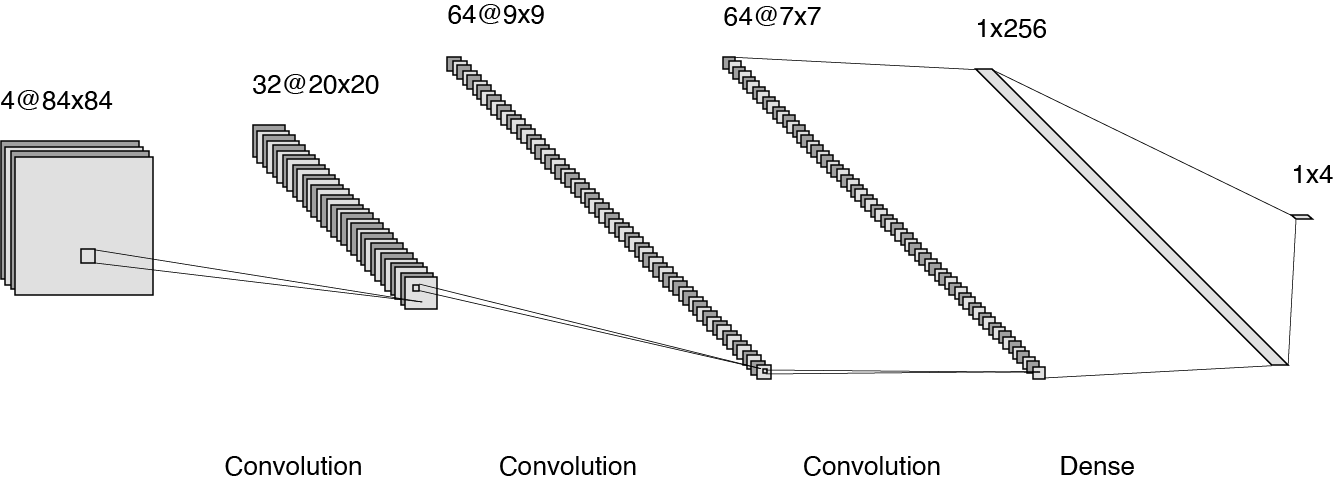
\includegraphics[width=0.75\textwidth]{chapters/chapter4/images/cnn.png}
	\caption{CNN Architecture
		\label{fig:project-dqn}
	}
\end{figure}

The above architecture was decided upon after reading different papers which implemented the agent. In the original DQN paper by Mnih et al. (2013) \cite{dqn} they proposed a slightly smaller network with only two convolutional layers. In papers released later, the network architecute was deepened, as deeper networks have shown to perform better in control tasks such as Atari. An additional factor to take into account was that the input image was already quite small at 84x84 pixels and as such, by using a very deep network could lead to having lots of dead filters due to the learning rate.

In this project, there was much room to explore network architectures. One area which was not explored but would be promising is using pooling layers. These have been shown to increase performance with rotational/position feature extraction which would be important for some of the more complex Atari games that require fine control such as Pitfall.

Overall, OpenAI Gym was an excellent choice for this project, it provided an excellent abstraction of the environment, exposing an API that could be used as necessary. Being able to just focus on the implementation of the agent provided more research time initially, and more time for performing a variety of tests for hyperparamter choice and network architecture. The following section will focus on the details of the DQN algorithm.

\subsection{DQN}
In this section, the details on how the DQN agent was implemented, along with the hyperparamters used during training. It was the area that the most difficult to implement in this project, primarily since Q-Networks are very sensitive to hyperparamter choice and implementation. During devleopment of the project, many iterations of the algorithm were tried until a setup that evaluated well with all the games in the test setup.

In the 2013 paper authored by DeepMind \cite{dqn}, they described the error function as the following. \textit{``We fixed all positive rewards to be 1 and all negative rewards to be $-1$, leaving 0 rewards unchanged''}. It was initially difficult to interpret, nevertheless, after reading some implementations of the algorihtm and Medium articles, it was clear that one such use the Huber loss before computing the gradients for updating the network. The Huber loss \ref{def:huber} is used is most good implementations of the DQN algorithm and has shown to reach a similar level of performance.

\begin{defn}
	Huber loss function.

	\begin{equation}
		L(a)=\begin{cases}
			\frac{1}{2}a^2,          & \text{for $\abs{a} \leq 1$}, \\
			(\abs{a} - \frac{1}{2}), & \text{otherwise}.
		\end{cases}
	\end{equation}
	\label{def:huber}
\end{defn}

Another aspect of the DQN algorithm that up to this point, we have not discussed in the report. That is of an idea of a \textit{``frame-skip''}. We have already talked about the frame-stack which is a rolling history of the past 4 frames which is used for forward passes through the network. While a frame-skip is when we take an action in the environment, then for a series of $k$ frames we perform the last action taken. This is very important and the frame-skip hyperparameter has been shown to be strong determining factor in the performance of algorithms when playing Atari \cite{braylan2015frame}.

A small note with the frameskip hyperparameter is that it was not kept the same for all the games that was tested. In the game Space Invaders it the frameskip was changed from $k = 4$ to $k = 3$. The reason for this was that the bullets (fired by both the aliens and player) flash every fourth frame; by using a frameskip of 4 it means that the bullets would never be visible during training. This was the only changed hyperparameter, all others were kept the same.

\begin{figure}[htbp]
	\centering
	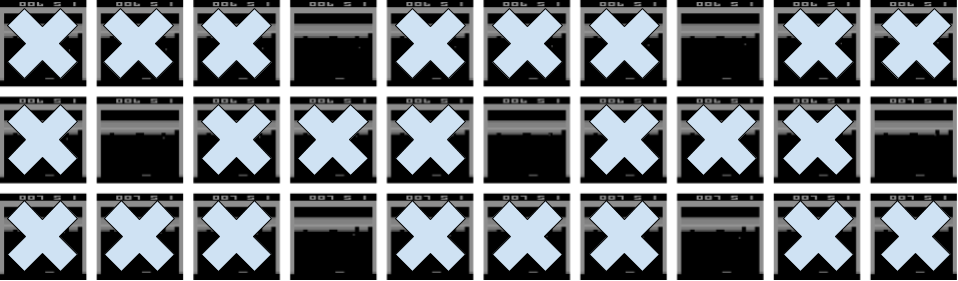
\includegraphics[width=0.75\textwidth]{chapters/chapter4/images/frameskip.png}
	\caption{Frameskip on Atari Breakout
		\label{fig:frameskip}
	}
\end{figure}

Figure \ref{fig:frameskip} shows how frames are sampled using frameskips. Using a frameskip, $k = 4$, as shown in the figure, we use every fourth frame from the game. If we denote every `seen' frame (those frames without the cross) as $x_1, x_2, \hdots, x_7$ then our first input, $s_1$, to the network will be $(x_1, x_2, x_3, x_4)$ and the the following input, $s_2$, would be $(x_2, x_3, x_4, x_5)$. An important observation of this method is that the states are overlapping in consecutative forward passes. It means that we provide the informtion to the network in order to predict the movement of the ball, such that we can move the paddle under the ball in time.

Another important consideration in the DQN algorithm is that of ``cold-starts''. This is when the environment is initalised and always starts from the same state. The worry with the cold starts is that the agent may not learn to look at a state and choose the optimal action, rather, it learns to cheat and learn a sequence of actions. This would lead to poor generalisation in the environment.

A solution to the problem of ``cold starts'' is to take between 0 and $k$ \texttt{NOOP} (No operation/No action) actions, sampled uniformly at random when the environment is initalised, putting the  environment in a slightly different state every time. This means that it would be more difficult for the agent to cheat in the environment by learning a set of actions from a starting state. The original DQN paper \cite{dqn} used $k = 30$ which was the value used in this project.

On the otherhand, recent reviews have cast doubt over the effectiveness of the \texttt{NOOP} actions helping the problem of cold starts. One example of this was a paper by M. C. Machado et al. (2017) \cite{machado2017revisiting} which argued that the \texttt{NOOP} sequence was not as effective as previously thought. Instead, it is proposed that it would be better to instead enforce random actions to be taken while the agent is being trained. By doing this, it adds a factor of stochasticity to the environment which also prevents the cold start problem.

\section{Visualisation}

Another important part of this project is the CNN visualisation. It was descirbed in section \ref{bg:sec:cnn-vis} however, in this section we will go into more detail about how it was implemented. It will first descirbe the motivation behind the choice of following a client-server architecture and then show the architecture diagramatically. Additionally, it covers some of the problems that were encountered during devleopment and how they were overcome.

The main consideration for this part of the project was how the model was executed, for which there was two options.

\begin{itemize}
	\item Executing the model in browser (using Tensorflow.js)
	\item Server-client architecture, the trained model executes on the server, sending updates to client.
\end{itemize}

Firstly, since this project used Tensorflow, programmed in Python, we could have loaded the trained model in Tensorflow.js and executed the model directly in the browser. However, for this approach to be viable, we would need to have also loaded the emulator in the browser in order to generate the frames of the game, this would require more engineering work. Additionally, not all client machines would be able to handle processing forward passes of the model.

Therefore, a client-server architecture was implemented instead using WebSockets to perform communication. The client would initiate the connection with the server and request a new environment. The server would take requests from the client for performing actions such as, running the model, performing a single step in the model; then sending the states back to the client over the socket. The main benefit of using Websockets is that it provides full-duplex communication channels over a single TCP connection, it reduces the overhead for sending messages between client and server (unlike using standard HTTP requests) and means that we can run the model at high frame rates (usually at least 30 FPS).

\begin{figure}[htbp]
	\centering
	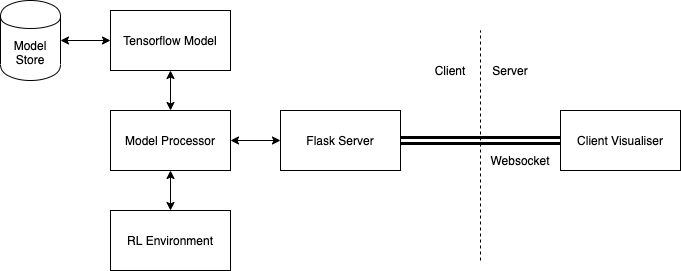
\includegraphics[width=0.70\textwidth]{chapters/chapter4/images/VizSystem.png}
	\caption[Visualisation system architecture]{Visualisation system architecture which shows how data flows between the major components. The top of the diagram show the server. Websocket commands are processed in the Flask server and delegated to either the tensorflow model or the environment by the Model Processor. The client can choose the model to visualise based on those available in the Model Store. The websocket established between client and server performs all the necessary transfer of information and the client is purley drawing the generated visualisation on the client screen.
		\label{fig:viz-system-arch}
	}
\end{figure}


The visualisation of the CNN also includes the raw filters and their activations. In order to visualise the filters, a forward pass of the network is performed using the current state. We store the history of the pass which includes the activations of each layer of the network (and of each filter), and importantly the resulting Q-values which are used to determine the best action to take given the current state. All this information is packaged into a predefined JSON format and sent over the socket to the client. The client parses this information and draws the pre-processed frame, the filters of the selected convolutional layer and the Q-values for each action. We also plot the Q-value of the chosen action over the past 50 frames, this allows the user to see if the agent is predicting a future reward. Figure \ref{fig:q-value-plot} shows how these Q-values are plotted, we see a slow rise, showing the agent is confident in the series of actions and then a sharp drop when the agent recieved the reward.

In Figure \ref{fig:q-value-plot}, the first screenshot show the ball moving upwards towards the row of bricks. At this point the network is confident in the series of actions and it is expecting a reward (show by point A in the plot). The second screenshot shows the ball has just broken a brick, at this point the agent recieves the reward and the Q value has a sudden and sharp drop (shown by point B). Finally, point C shows that the Q-value has dropped down to its original value (corresponding to the third screenshot as the ball is travelling down to the paddle). This shows that the agent can learn to predict a complex series of events.


\begin{figure}[htbp]
	\centering
	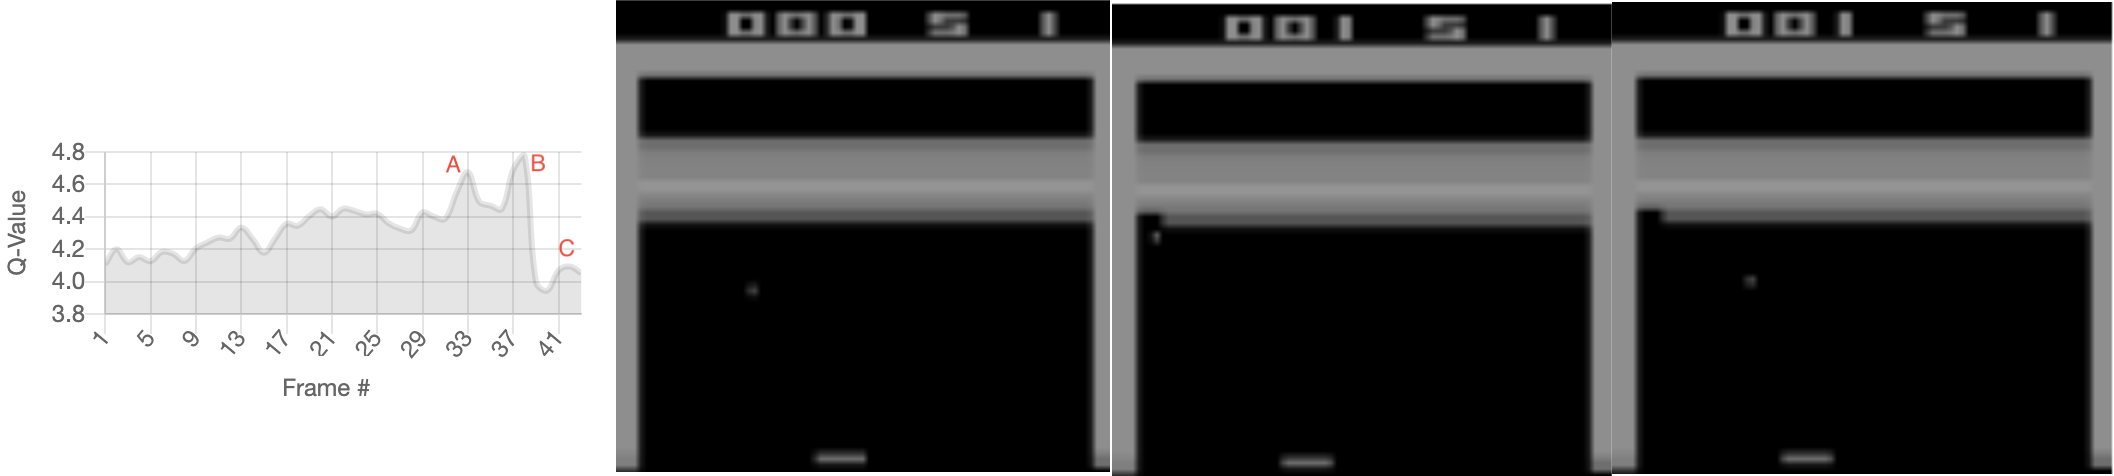
\includegraphics[width=1\textwidth]{chapters/chapter4/images/qvalue-plot.png}
	\caption[Q-Value function visualisation]{The Q-value function output is shown in the left-most figure (the max Q-value from the network predictions), shown over a 45 frame history. The next three screenshots correspond to the frames labelled by A, B and C in the left-most figure respectively.
		\label{fig:q-value-plot}
	}
\end{figure}

Finally, the web server which handles the emulation of the environment and running the model uses a selection of commands (which are sent over the socket) in order for a client to control the environment. The server runs Flask which is a micro-framework for creating web applications. The framework was chosen since it is lightweight, extensible and quick to setup. Additionally, it had a module which supported WebSockets, making the implementation of the visualisation easier as it provided an abstraction from the details of maintaining the Socket.